% =============================================================================
% Resumo expandido — EST613 Estatística Bayesiana (UFV)
% Classificação bayesiana dinâmica de proficiência em Biologia
% JPGTEIXEIRA — compilar com: pdflatex resumo_expandido.tex (duas vezes)
% Figuras lidas de ../results/ (geradas pela main.R)
% =============================================================================
\documentclass[12pt,a4paper]{article}

\usepackage[utf8]{inputenc}
\usepackage[T1]{fontenc}
\usepackage[brazil]{babel}
\usepackage{mathptmx}                 % fonte Times
\usepackage[a4paper,margin=2.5cm]{geometry}
\usepackage{amsmath,amssymb}
\usepackage{graphicx}
\usepackage{booktabs}
\usepackage{caption}
\usepackage[hidelinks]{hyperref}
\usepackage{setspace}
\usepackage[round,authoryear]{natbib}

\graphicspath{{../results/}}
\captionsetup{font=small,labelfont=bf}
\setlength{\parskip}{0pt}
\onehalfspacing

\begin{document}

% -----------------------------------------------------------------------------
% Título e identificação
% -----------------------------------------------------------------------------
\begin{center}
  {\large\bfseries Classificação bayesiana dinâmica de proficiência em Biologia:\\
  níveis do tipo PAEBES atualizados ao longo do ano letivo}\\[0.8em]
  João Paulo Gusmão Teixeira\\
  {\small Programa de Pós-Graduação em Genética e Melhoramento -- Universidade Federal de Viçosa\\
  EST613 -- Estatística Bayesiana -- Profa. Camila Ferreira Azevedo}
\end{center}

% -----------------------------------------------------------------------------
\section{Introdução}
% -----------------------------------------------------------------------------

O Programa de Avaliação da Educação Básica do Espírito Santo (PAEBES) é utilizado para
monitorar a aprendizagem no estado e classifica os estudantes em quatro padrões de desempenho:
Abaixo do Básico, Básico, Proficiente e Avançado. Por se tratar de uma avaliação externa
aplicada poucas vezes, ao longo do ano letivo a escola dispõe apenas das notas atribuídas pelos
professores. Essas notas, entretanto, não refletem somente a proficiência do aluno, pois
dependem também da escola de origem e do rigor do professor que aplica cada avaliação
\citep{zitzmann2025}. Além disso, a média simples, adotada pelas escolas, atribui o mesmo peso
a avaliações antigas e recentes e não informa o grau de confiança na proficiência estimada.

Nesse contexto, a abordagem bayesiana constitui uma ferramenta adequada para tratar essas
questões. A nota do histórico escolar, disponível antes do início do ano, pode ser utilizada
como informação a priori \citep{vanmoere2020}, enquanto cada avaliação do ano compõe a
verossimilhança. Desse modo, a distribuição a posteriori fornece, a cada avaliação, a
probabilidade de o aluno pertencer a cada nível. Ao se admitir que a proficiência varia no
tempo, o modelo utiliza um conceito similar ao do filtro de Kalman \citep{kalman1960}, no qual
a posteriori de uma avaliação é a priori da seguinte.

% -----------------------------------------------------------------------------
\section{Objetivo}
% -----------------------------------------------------------------------------

Propor e avaliar um modelo bayesiano que classifique o padrão de desempenho dos alunos em
Biologia a partir do seu histórico escolar e das notas ao longo do ano letivo.

% -----------------------------------------------------------------------------
\section{Metodologia}
% -----------------------------------------------------------------------------

\textbf{Dados simulados.} Foram simulados 120 alunos da 1ª série do Ensino Médio, resultantes
do cruzamento de três níveis de entrada (proficiência média de 35, 55 e 85) com quatro
trajetórias ao longo do ano (evolução, involução, estagnação e oscilação), com 10 alunos por
perfil e 9 avaliações por aluno (três trimestres, cada um com duas provas e um trabalho). Os
alunos são provenientes de cinco escolas de origem, das quais uma (E5) atribui notas 12 pontos
acima da proficiência, e o professor de origem é conhecido para cerca de 40\% deles. Na escola
atual, há três professores, identificados pelo rigor: PR (rigoroso, $-10$), PM (mediano, 0) e
PF (flexível, $+8$). Como a aprovação exige nota $\ge 60$, o aluno cujo histórico seria inferior
a esse valor ingressa com nota 60, embora mantenha a proficiência real, situação que ocorreu
com 60 dos 120 alunos.

\textbf{Modelo e verossimilhança.} Seja $\theta_{it}$ a proficiência do aluno $i$ na
avaliação $t$. As notas do ano ($y_{it}$) e a nota do histórico ($h_i$) são modeladas como
\begin{equation}
  y_{it} \sim \mathcal{N}(\theta_{it} + \delta_{a(i)},\ \sigma^2), \qquad
  h_i \sim \mathcal{N}(\theta_{i1} + \gamma_{e(i)} + \delta_{p(i)},\ \sigma_h^2), \qquad
  \theta_{it} = \theta_{i,t-1} + \eta_{it},\ \ \eta_{it} \sim \mathcal{N}(0, \omega^2),
\end{equation}
em que $\delta_{a(i)}$ representa o efeito do professor atual do aluno $i$, $\gamma_{e(i)}$ e
$\delta_{p(i)}$ representam os efeitos da escola e do professor de origem, $\sigma^2$ e
$\sigma_h^2$ são as variâncias dos erros das notas do ano e do histórico, e $\eta_{it}$ é o
ruído da dinâmica, com variância $\omega^2$, que representa a variação da proficiência entre
avaliações consecutivas. Esse ruído aumenta a incerteza antes de cada avaliação, de modo que as
avaliações recentes recebem maior peso que as antigas. O histórico igual a 60 é tratado como
censurado, uma vez que se sabe apenas que o valor verdadeiro era $\le 60$. A verossimilhança é
\begin{equation}
  L = \prod_{i=1}^{120}\Big[\prod_{t=1}^{9}\phi\big(y_{it};\,\theta_{it}+\delta_{a(i)},\,\sigma^2\big)\Big]
  \,\phi\big(h_i;\,\mu_{h,i},\,s_i^2\big)^{1-d_i}\,
  \Phi\big((60-\mu_{h,i})/s_i\big)^{d_i},
\end{equation}
em que $d_i = 1$ quando $h_i = 60$ (histórico censurado) e $d_i = 0$ nos demais casos,
$\mu_{h,i} = \theta_{i1}+\gamma_{e(i)}+\delta_{p(i)}$ e $s_i^2 = \sigma_h^2$. Quando o professor
de origem é desconhecido, seu efeito não é imputado, mas integrado, isto é, $\delta_{p(i)}$ é
retirado de $\mu_{h,i}$ e sua variância é somada à do histórico, de modo que
$s_i^2 = \sigma_h^2 + \tau_{\text{prof}}^2$.

\textbf{Modelos comparados.} Foram comparados três modelos. O M0 corresponde à média simples
das notas. O M1 consiste em uma atualização Normal--Normal conjugada, sem $\gamma$ e $\delta$,
que utiliza a nota do histórico, sem ajuste, como média a priori e adota variâncias fixas,
obtidas do desenho da simulação: $\sigma = 6$ corresponde ao erro simulado das provas,
$\sigma_0 = 10$ acrescenta ao erro do histórico os efeitos de escola e professor que o M1 não
desconta, e $\omega = 3$ aproxima a mudança média por avaliação. Essa escolha favorece o M1 e
torna a comparação conservadora. O M2 é o modelo completo, hierárquico, ajustado por MCMC
(NUTS) no Stan \citep{carpenter2017}, com $\gamma_e \sim \mathcal{N}(0, \tau_{\text{esc}}^2)$ e
$\delta \sim \mathcal{N}(0, \tau_{\text{prof}}^2)$. Os efeitos dos professores atuais foram
restritos a somar zero, o que fixa a escala e garante a identificabilidade do modelo. As
distribuições a priori foram $\tau \sim \text{half-Normal}(0, 10)$,
$\sigma \sim \text{half-Normal}(0, 10)$, $\omega \sim \text{half-Normal}(0, 5)$,
$\sigma_h \sim \text{Gama}(2;\,0{,}2)$ e $\theta_{i1} \sim \mathcal{N}(50, 25^2)$. Como há
poucos grupos, a priori de $\tau$ foi substituída por uma half-Cauchy$(0, 5)$ em uma análise de
sensibilidade \citep{gelman2006}.

\textbf{Inferência e avaliação.} Antes do ajuste, foi realizada uma checagem preditiva a
priori, com notas simuladas apenas a partir das distribuições a priori. Foram utilizadas quatro
cadeias de 2.000 iterações, das quais 1.000 de aquecimento. A convergência foi avaliada pelos
diagnósticos de Gelman--Rubin, Geweke e Heidelberger--Welch, pelo tamanho efetivo de amostra
(ESS), pelo erro de Monte Carlo (MCSE), pela autocorrelação e pelo número de transições
divergentes, e os intervalos de credibilidade foram obtidos como HPD de 95\%. Com limites em
40, 60 e 80, a probabilidade de cada nível corresponde à proporção de amostras de
$\theta_{it}$ (truncado em [0, 100]) em cada faixa. Isso equivale a um teste de hipóteses
bayesiano em que cada nível é uma região do espaço paramétrico, de forma análoga às
probabilidades de desempenho superior empregadas na recomendação de cultivares
\citep{dias2022}. Foram comparadas duas regras de classificação: o nível de maior
probabilidade e um limiar, segundo o qual o aluno só muda de nível quando a probabilidade do
novo nível supera 0,7. O ajuste foi avaliado sem o uso dos valores verdadeiros, por meio da
comparação do M2 com a mesma estrutura sem $\gamma$ e $\delta$, pelo DIC
\citep{spiegelhalter2002} e pela validação cruzada com exclusão de um aluno por vez (LOO;
\citealp{vehtari2017}). Nesta, a verossimilhança de cada aluno integra seus $\theta_{it}$ de
forma exata pelo filtro de Kalman, o que permite avaliar a capacidade do modelo de prever as
notas de um aluno novo. A adequação foi avaliada por verificação preditiva a posteriori em três
níveis: global (todas as notas), de grupo (professor e escola de origem) e individual (variação
das notas de cada aluno). Por fim, os valores verdadeiros da simulação foram utilizados para
medir a taxa de acerto da classificação, o número de trocas de nível por aluno e a proporção
de mudanças reais de nível não detectadas.

% -----------------------------------------------------------------------------
\section{Resultados e discussão}
% -----------------------------------------------------------------------------

\textbf{Construção e convergência do M2.} O modelo final foi obtido em quatro etapas, com a
alteração de um elemento por vez. Sem a restrição de soma zero, o modelo não era
identificável, razão pela qual as cadeias apresentaram 9 transições divergentes e os efeitos
dos professores foram estimados com deslocamento ($+12{,}0$, $+4{,}3$ e $-5{,}5$, ante os
valores verdadeiros de $+8$, 0 e $-10$). A restrição corrigiu as estimativas. A priori Gama,
que afasta $\sigma_h$ de zero, elevou o ESS desse parâmetro de 307 para 854, e a
parametrização não centrada de $\delta_a$ ($\delta = \tau z$) evitou a geometria em funil que
ocorre quando $\tau \to 0$. No modelo final, sob ambas as prioris para $\tau$, o Gelman--Rubin
foi $\le 1{,}01$, o ESS mínimo superou 540, ocorreu uma transição divergente em 4.000 e os
testes de Heidelberger--Welch foram aprovados, com exceção de $\gamma_{E2}$ em uma das quatro
cadeias. No diagnóstico de Geweke, 5 (half-Normal) e 10 (half-Cauchy) dos 52 testes
apresentaram $|z| > 1{,}96$.

\textbf{Ajuste e capacidade preditiva.} Os dois critérios favoreceram o modelo com efeitos de
escola e professor (DIC de 7.835, ante 7.939, e diferença de ELPD no LOO por aluno de 41,1, com
erro-padrão de 7,6), que previu melhor as notas de 93 dos 120 alunos. O LOO por nota foi
descartado, pois, como cada nota possui um parâmetro latente próprio, 59 das 1.200 notas
apresentaram Pareto-$k > 0{,}7$. No LOO por aluno, apenas quatro alunos superaram esse limite,
e a diferença de ELPD se manteve após sua exclusão (45,3).

\textbf{Adequação do modelo.} A checagem preditiva a priori indicou que as distribuições a
priori geram notas na escala esperada (mediana de 50), embora 9\% dos valores simulados fiquem
fora do intervalo de 0 a 100 (percentis de 1\% e 99\% iguais a $-20$ e 120). Assim, essas
distribuições são pouco informativas, mas não respeitam os limites da escala. A verificação
preditiva a posteriori reproduziu os dados nos três níveis avaliados: média e desvio-padrão
globais ($p = 0{,}47$ e $0{,}56$), diferença entre professores ($p = 0{,}45$) e entre escolas
no histórico ($p = 0{,}66$) e variação das notas de cada aluno ($p = 0{,}60$). A exceção foi a
nota máxima ($p = 1{,}00$), uma vez que o modelo gera notas acima de 100, problema já observado
na checagem a priori, por tratar como normais as notas censuradas em 100 (28 das 1.080).
Portanto, embora o M2 tenha convergido e apresentado o melhor desempenho na comparação,
persiste uma falta de ajuste identificável, o que evidencia que a convergência e o desempenho
relativo não garantem adequação.

\textbf{Classificação.} O M2 classificou corretamente cerca de 83\% dos registros, ante 66\%
da média simples e 68\% do M1 (Tabela~\ref{tab:modelos}). O ganho decorreu principalmente da
estimação dos efeitos de escola e professor. Com o professor rigoroso (PR), a taxa de acerto
passou de 55\% (M0) e 59\% (M1) para 79\% (M2), enquanto, com o professor mediano (PM), os
modelos apresentaram desempenho semelhante (79\% a 85\%). A regra do limiar reduziu as trocas
de nível espúrias de 0,60 para 0,36 por aluno, porém deixou de detectar mais mudanças reais
(40\%, ante 31\%). A substituição pela half-Cauchy praticamente não alterou os resultados.
Esse padrão corrobora \citet{zitzmann2025}, segundo os quais a incorporação de informação
prévia melhora a avaliação individual apenas quando essa informação é pouco viesada. No
presente estudo, o M1, que utiliza o histórico sem ajuste, obteve acerto semelhante ao da
média simples, ao passo que o M2, ao estimar e descontar os efeitos de escola e professor,
apresentou o maior ganho. De modo semelhante, \citet{kaplan2023} mostraram que dados
históricos heterogêneos são mais bem aproveitados quando o grau de empréstimo de informação é
estimado.

\begin{table}[h]
  \centering
  \caption{Desempenho da classificação dos 120 alunos ao longo das 9 avaliações.}
  \label{tab:modelos}
  \small
  \begin{tabular}{lccc}
    \toprule
    Modelo & Acerto (\%) & Trocas por aluno & Mudanças não detectadas (\%) \\
    \midrule
    M0 -- média simples              & 66,4 & 0,58 & 48,1 \\
    M1 -- limiar 0,7                 & 67,9 & 0,62 & 38,3 \\
    M2 -- limiar 0,7                 & 82,8 & 0,36 & 39,5 \\
    M2 -- maior probabilidade        & 84,7 & 0,60 & 30,9 \\
    M2 -- limiar 0,7 (half-Cauchy)   & 82,7 & 0,35 & 40,7 \\
    \bottomrule
    \multicolumn{4}{l}{\footnotesize Trocas reais: 1,55 por aluno, com 81 dos 120 alunos mudando de nível ao longo do ano.}
  \end{tabular}
\end{table}

\textbf{Efeitos, \textit{partial pooling} e hipóteses.} O M2 recuperou os efeitos simulados,
com estimativa de $+11{,}5$ para a escola E5 (HPD 95\%: 7,0 a 15,6, com valor verdadeiro de
$+12$) e de $-9{,}1$, $+0{,}9$ e $+8{,}3$ para os professores PR, PM e PF (valores verdadeiros
de $-10$, 0 e $+8$). Como teste de hipóteses bayesiano, obteve-se
$P(\delta_{\text{PR}} < 0 \mid \text{dados}) = 1{,}00$ e
$P(\delta_{\text{PF}} > 0 \mid \text{dados}) = 1{,}00$, enquanto o professor mediano apresentou
probabilidade de 0,84 de estar na região de equivalência prática (ROPE) de $\pm 2$ pontos.
Para os professores de origem, o efeito do compartilhamento parcial de informação
(\textit{partial pooling}) foi evidente, pois, em relação à estimativa obtida apenas com os
próprios alunos, a do M2 foi reduzida em direção a zero por um fator de 0,67 a 0,75 para
professores com um aluno e de 0,87 a 0,89 para professores com cinco alunos, conforme previsto
pela teoria ($\tau^2 / (\tau^2 + \sigma_h^2/n)$). A Figura~\ref{fig:trajetorias} ilustra esse
mecanismo: com o professor flexível, M0 e M1 acompanham as notas infladas, enquanto o M2
desconta o efeito do professor e se aproxima da trajetória verdadeira.

\begin{figure}[h]
  \centering
  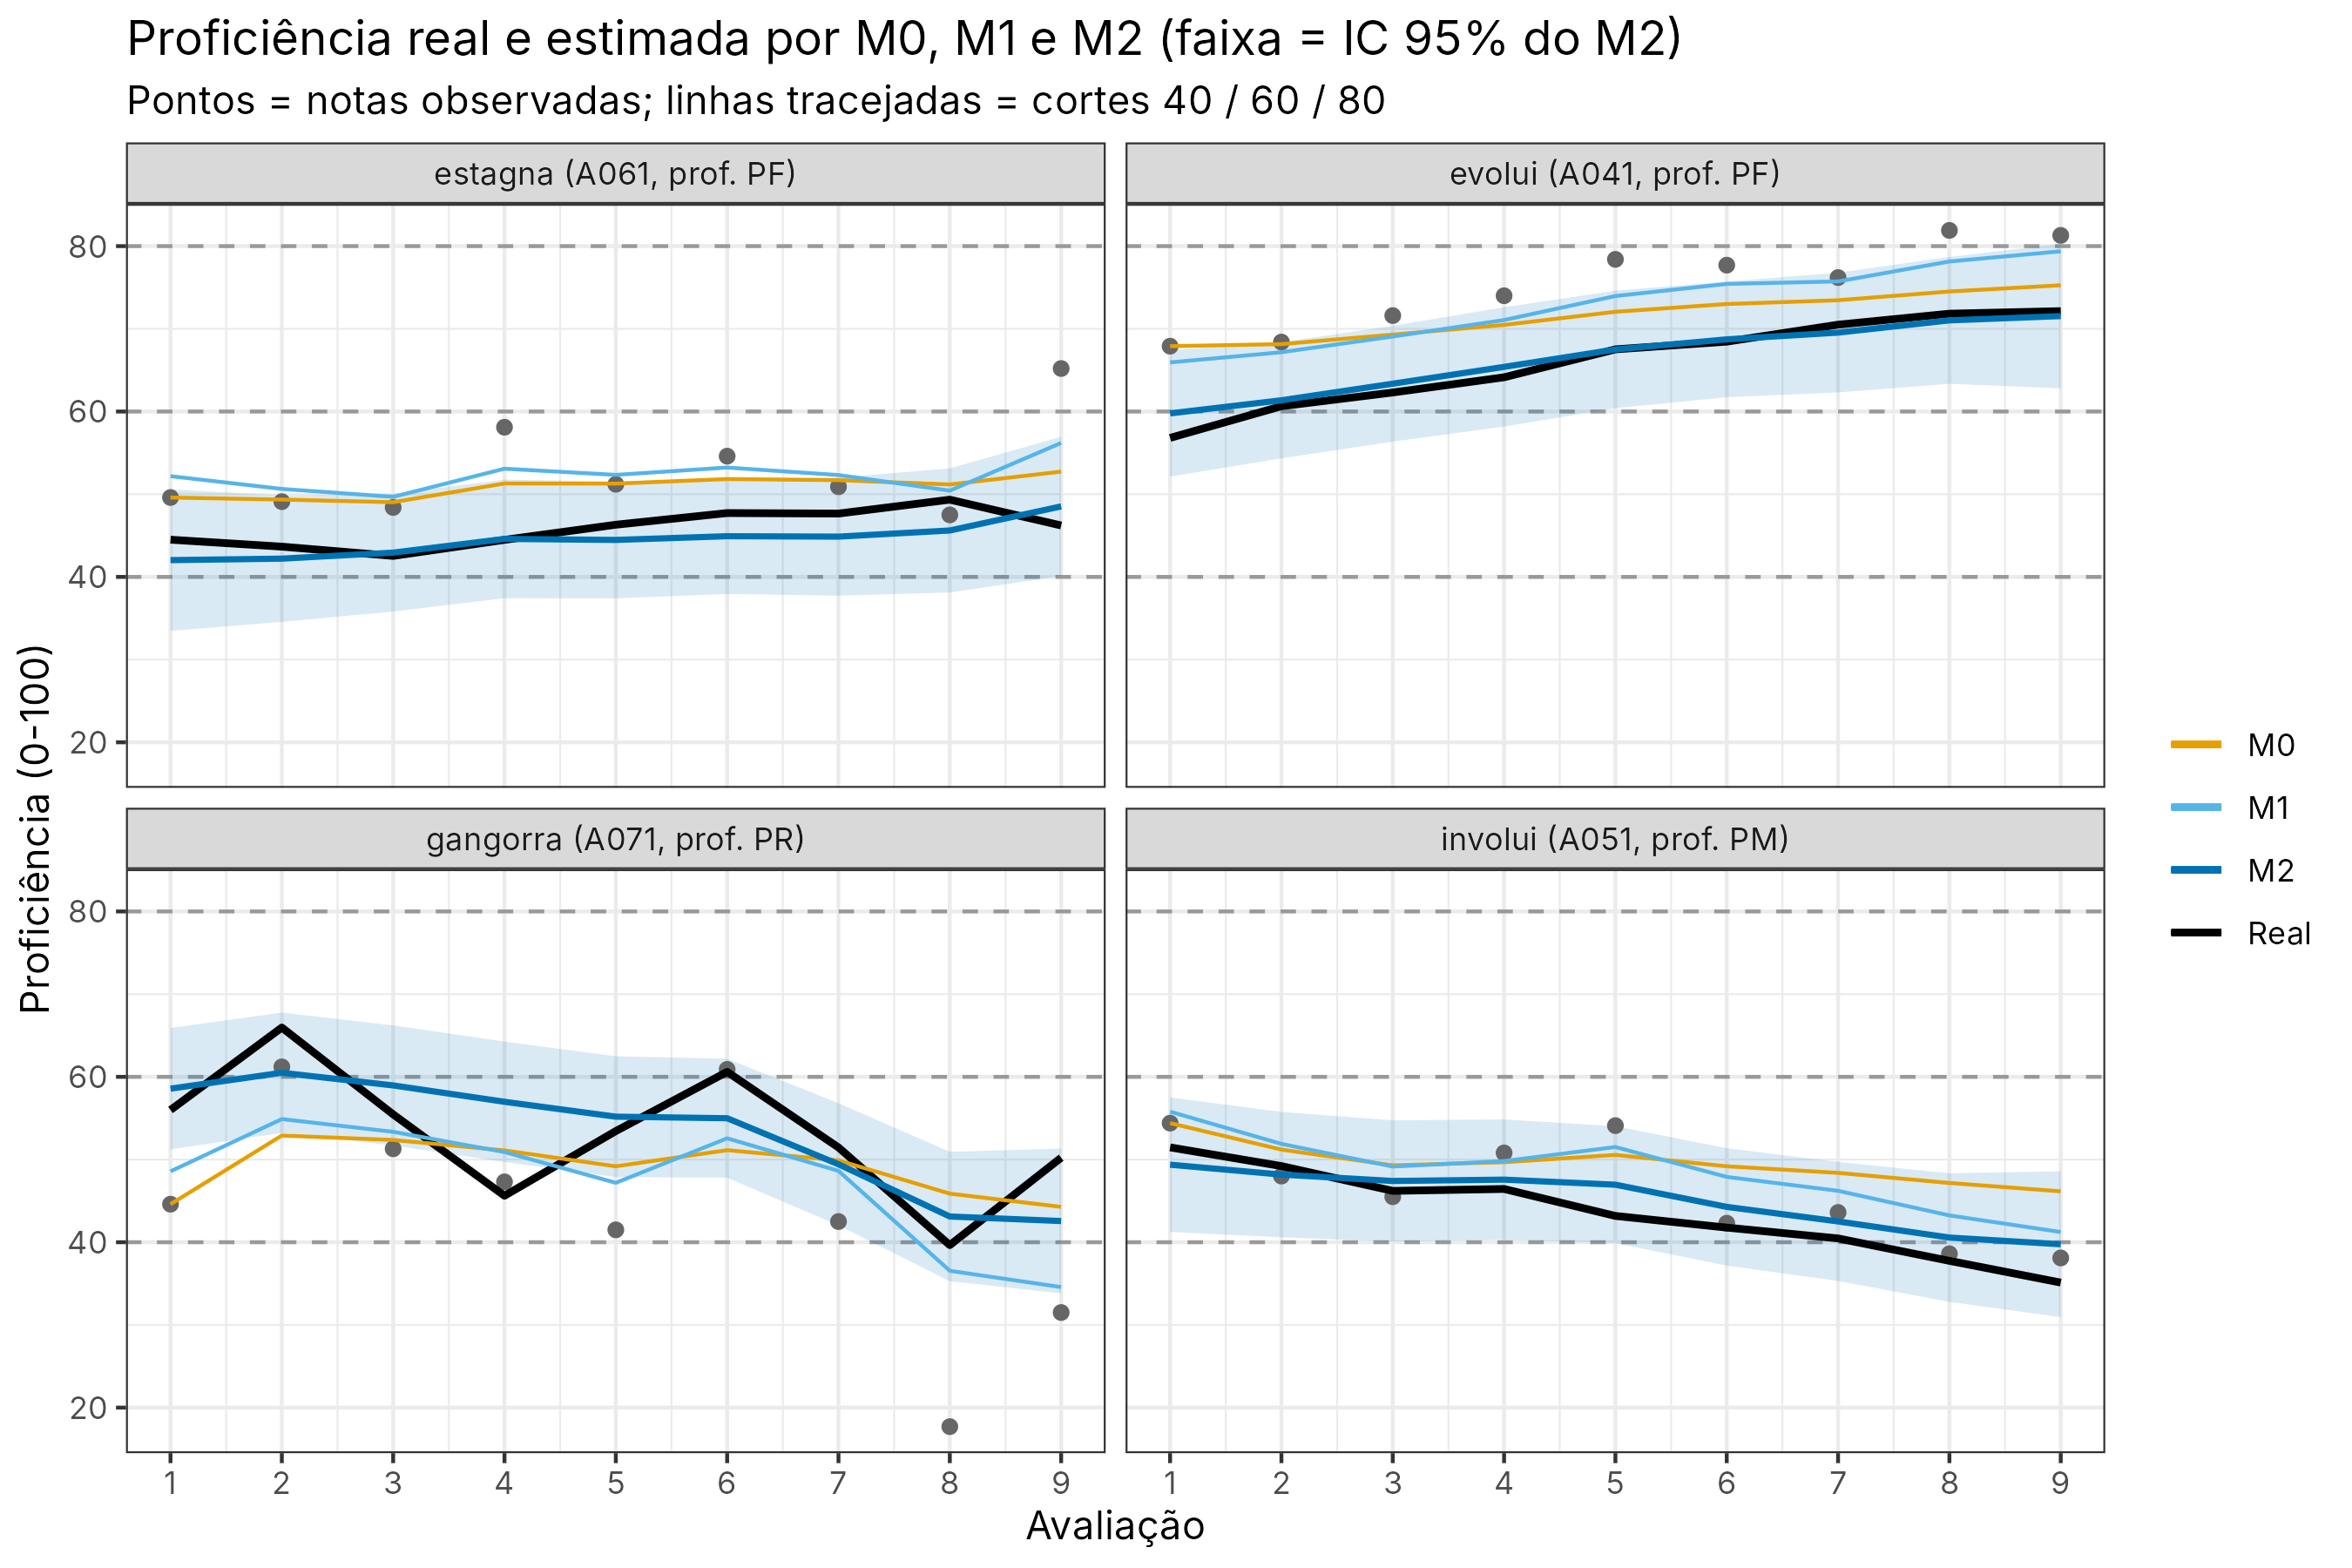
\includegraphics[width=0.75\textwidth]{fig1_trajetorias.png}
  \caption{Proficiência verdadeira (preto) e estimada por M0, M1 e M2 para um aluno de cada
  trajetória. A faixa corresponde ao intervalo de credibilidade de 95\% do M2, os pontos, às
  notas observadas, e as linhas tracejadas, aos limites entre os níveis.}
  \label{fig:trajetorias}
\end{figure}

Ressalta-se que os resultados se baseiam em uma única réplica simulada. Além disso, a separação
entre o rigor do professor e o nível da turma exige conexão entre os dados, como alunos que
trocam de professor, professores com várias turmas ou uma referência externa comum.

% -----------------------------------------------------------------------------
\section{Conclusão}
% -----------------------------------------------------------------------------

O classificador bayesiano dinâmico que considera a escola de origem e o rigor do professor
classificou os alunos melhor que a média simples e identificou mais mudanças de nível ao longo
do ano. O principal ganho decorreu da estimação dos efeitos de escola e professor, resultado
confirmado pelo DIC e pela validação cruzada por aluno, critérios que não dependem dos valores
verdadeiros. Como o modelo utiliza apenas as notas já registradas pela escola, sua aplicação
não exige mudanças na rotina escolar. As próximas etapas consistem na aplicação a dados reais
da Secretaria de Educação do Espírito Santo e em duas extensões que preservam a lógica do
modelo. Com o histórico completo do Ensino Fundamental (6º ao 9º ano), a priori do 1º ano
passaria a ser a própria posteriori do modelo dinâmico ao fim do 9º ano, com maior peso para as
notas recentes. Com alunos que possuam tanto as notas escolares quanto o resultado no PAEBES, a
avaliação estadual serviria de referência externa comum, o que permitiria calibrar os efeitos
de escola e professor em termos absolutos e prever, pela distribuição preditiva, a
probabilidade de cada aluno atingir cada padrão de desempenho, como alerta precoce. Para isso,
será necessário relacionar a escala das notas escolares (0 a 100) à escala de proficiência do
PAEBES, de modo que a classificação seja realizada diretamente nos padrões de desempenho
oficiais.

% -----------------------------------------------------------------------------
% Referências
% -----------------------------------------------------------------------------
\begin{thebibliography}{9}
\setlength{\itemsep}{0pt}
\footnotesize

\bibitem[Carpenter et al.(2017)]{carpenter2017}
CARPENTER, B. et al. Stan: a probabilistic programming language.
\textit{Journal of Statistical Software}, v. 76, n. 1, p. 1--32, 2017.

\bibitem[Dias et al.(2022)]{dias2022}
DIAS, K. O. G. et al. Leveraging probability concepts for cultivar recommendation in
multi-environment trials. \textit{Theoretical and Applied Genetics}, v. 135,
p. 1385--1399, 2022.

\bibitem[Gelman(2006)]{gelman2006}
GELMAN, A. Prior distributions for variance parameters in hierarchical models.
\textit{Bayesian Analysis}, v. 1, n. 3, p. 515--534, 2006.

\bibitem[Kalman(1960)]{kalman1960}
KALMAN, R. E. A new approach to linear filtering and prediction problems.
\textit{Journal of Basic Engineering}, v. 82, n. 1, p. 35--45, 1960.

\bibitem[Kaplan et al.(2023)]{kaplan2023}
KAPLAN, D. et al. Bayesian dynamic borrowing of historical information with applications to
the analysis of large-scale assessments. \textit{Psychometrika}, v. 88, n. 1, p. 1--30, 2023.

\bibitem[Spiegelhalter et al.(2002)]{spiegelhalter2002}
SPIEGELHALTER, D. J. et al. Bayesian measures of model complexity and fit.
\textit{Journal of the Royal Statistical Society B}, v. 64, n. 4, p. 583--639, 2002.

\bibitem[Van Moere e Hanlon(2020)]{vanmoere2020}
VAN MOERE, A.; HANLON, S. A Bayesian approach to improving measurement precision over
multiple test occasions. \textit{Language Testing}, v. 37, n. 4, p. 482--502, 2020.

\bibitem[Vehtari et al.(2017)]{vehtari2017}
VEHTARI, A.; GELMAN, A.; GABRY, J. Practical Bayesian model evaluation using
leave-one-out cross-validation and WAIC. \textit{Statistics and Computing}, v. 27,
p. 1413--1432, 2017.

\bibitem[Zitzmann et al.(2025)]{zitzmann2025}
ZITZMANN, S. et al. Novick meets Bayes: improving the assessment of individual students in
educational practice and research by capitalizing on assessors' prior beliefs.
\textit{Educational and Psychological Measurement}, v. 85, n. 3, p. 483--506, 2025.

\end{thebibliography}

\end{document}
